\documentclass{report}
% PACKAGES %
\usepackage[english]{} % Sets the language
\usepackage[margin=2cm]{geometry} % Sets the margin size
\usepackage{fancyhdr} % Allows creation of headers
\usepackage{graphicx} % Enhanced package for including graphics/figures
\usepackage{float} % Allows figures and tables to be floats
\usepackage{amsmath} % Enhanced math package prepared by the American Mathematical Society
\usepackage{amssymb} % AMS symbols package
\usepackage{mathrsfs}% More math symbols
\usepackage{bm} % Allows you to use \bm{} to make any symbol bold
\usepackage{bbold} % Allows more bold characters
\usepackage{verbatim} % Allows you to include code snippets
\usepackage{setspace} % Allows you to change the spacing between lines at different points in the document
\usepackage{parskip} % Allows you alter the spacing between paragraphs
\usepackage{multicol} % Allows text division into multiple columns
\usepackage{units} % Allows fractions to be expressed diagonally instead of vertically
\usepackage{booktabs,multirow,multirow} % Gives extra table functionality
\usepackage{hyperref} % Allows hyperlinks in the document
\usepackage{rotating} % Allows tables to be rotated

\newcommand{\tab}{\-\hspace{1.5cm}}

% Set path to figure image files
\graphicspath{ {"/Users/mitch/Documents/Cal/2_2017_Spring/COMPSCI 289A - Intro to Machine Learning/HW04/Figures/"} }

% Create a header w/ Name & Date
\pagestyle{fancy}
\rhead{\textbf{Mitch Negus} 3032146443}

\begin{document}
\thispagestyle{empty}

{\bf {\large {COMPSCI 289A} Homework {4} \hfill Mitch Negus\\
		3/13/2017 						\hfill	3032146443}}\\\\


%%%%%%%%%%%%%%%%%%%%%%%%%%%%%%%%%% PROBLEM 1 %%%%%%%%%%%%%%%%%%%%%%%%%%%%%%%%%%
\section*{Problem 1}

\subsection*{1.)}

The gradient of the cost function $J(w)$ is given by
$$ \nabla_w J(w) = \nabla_w \left( \lambda |w|_2^2 - \sum_{i=1}^n{ y_i \ln s_i + (1-y_i) \ln (1-s_i)} \right) $$
$$ \nabla_w J(w) = \lambda \nabla_w(|w|_2^2) - \nabla_w \left(  \sum_{i=1}^n{ y_i \ln s_i + (1-y_i) \ln (1-s_i)} \right) $$
Using our result from homework 2, that $\nabla_x (x^TAx) = 2Ax$, we can state that $|w|_2^2 = w^T\mathbb{1}w$ and so $\nabla_x(|x|_2^2) = 2\mathbb{1}w = 2w$. Then
$$ \nabla_w J(w) = 2 \lambda w - \sum_{i=1}^n{\left( y_i  \nabla_w (\ln s_i )+ (1-y_i) \nabla_w \ln (1-s_i) \right)}$$
$$ \nabla_w J(w) = 2 \lambda w - \sum_{i=1}^n{\left( \frac{y_i}{s_i}\nabla_w s_i - \frac{1-y_i}{1-s_i} \nabla_w s_i \right)} $$
We know $s_i = s(X_i \cdot w) = 1/(1 + e^{-X_i \cdot w})$, so 
$$ \nabla_w s_i = \nabla_w \left( \frac{1}{1 + e^{-X_i \cdot w}} \right) $$
$$ \nabla_w s_i = \frac{X_i e^{-X_i \cdot w}}{(1 + e^{-X_i \cdot w})^2} $$
$$ \nabla_w s_i = X_i s_i \frac{e^{-X_i \cdot w}}{1 + e^{-X_i \cdot w}} $$
$$ \nabla_w s_i = X_i s_i (1-s_i) $$
and thus 
$$ \nabla_w J(w) = 2 \lambda w - \sum_{i=1}^n{\left( \frac{y_i}{s_i}(X_i s_i (1-s_i)) - \frac{1-y_i}{1-s_i} (X_i s_i (1-s_i)) \right)} $$
$$ \nabla_w J(w) = 2 \lambda w - \sum_{i=1}^n{\left( y_i X_i (1-s_i) - (1-y_i) X_i s_i  \right)} $$
$$ \nabla_w J(w) = 2 \lambda w - \sum_{i=1}^n{\left( y_i X_i - y_i X_i s_i  - X_i s_i + y_i X_i s_i \right)} $$
$$ \nabla_w J(w) = 2 \lambda w - \sum_{i=1}^n{\left( y_i X_i - X_i s_i \right)} $$
$$ \nabla_w J(w) = 2 \lambda w - \sum_{i=1}^n{\left( y_i - s_i \right)X_i} $$
$$\boxed{ \nabla_w J(w) = 2 \lambda w - X^T(y-s) }$$


\subsection*{2.)}

The Hessian of $J(w)$ is 
$$ \nabla_w^2 J(w) = \nabla_w(\nabla_w J(w)) = \nabla_w ( 2 \lambda w - X^T(y-s) ) $$
$$ \nabla_w^2 J(w) = 2 \lambda\mathbb{1} - \nabla_w \left(\sum_{i=1}^n{\left( y_i - s_i \right)X_i}\right) $$
$$ \nabla_w^2 J(w) = 2 \lambda\mathbb{1} + \sum_{i=1}^n{\nabla_w (s_i X_i)} $$
$$ \nabla_w^2 J(w) = 2 \lambda\mathbb{1} + \sum_{i=1}^n{\nabla_w(s_i)X_i} $$
$$ \nabla_w^2 J(w) = 2 \lambda\mathbb{1} + \sum_{i=1}^n{s_i(1-s_i)X_i X_i^T} $$
$$\boxed{ \nabla_w^2 J(w) = 2 \lambda\mathbb{1} + X^T \Omega X}, \text{ where } 
									\Omega = \begin{bmatrix} s_1(1-s_1) & 0 & \hdots & 0 \\
														0 & s_2(1-s_2) & \hdots & 0 \\
														\vdots & \vdots & \ddots & \vdots \\
														0 & 0 & \hdots & s_n(1-s_n)
											\end{bmatrix} $$
											


\subsection*{3.)}

Expanding the Taylor series as discussed in lecture and considering only the first 2 terms as a quadratic approximation to the cost function at our point $w$, 
$$ J(w') = J(w) + (\nabla J(w))(w'-w) + ... \; .$$
We can find a minimum for the new point, $w'$, by taking the gradient of $J(w')$, and setting it equal to zero:
$$ \nabla J(w') = \nabla J(w) + (\nabla^2 J(w))(w'-w) + O(|w'-w|^2) $$
Disregarding small terms,
$$ 0 = \nabla J(w) + (\nabla^2 J(w))(w'-w) $$
$$ 0 = \nabla J(w) + (\nabla^2 J(w))(w'-w) $$
$$ -\nabla^2 J(w) w' = \nabla J(w)  - \nabla^2 J(w) w $$
$$ w' = w - (\nabla^2 J(w))^{-1}(\nabla J(w)) .$$
Since we would like to avoid calculating the inverse of $\nabla^2 J(w))$, we can substitute $e$ in for the second term so that $w'$ would be given by: 
$$ w' = w + e , \text{ where } e \text{ is the solution to the equation } (\nabla^2 J(w))e = -\nabla J(w) .$$
Then, modifying the solution for $w'$ to be an update rule, we can incorporate our calculated gradient and Hessian to state
$$\boxed{ w \leftarrow w + e , \text{ where } e \text{ is the solution to the equation } ( X^T \Omega X + 2\lambda\mathbb{1} ) e = X^T(y-s) - 2 \lambda w }.$$.


\subsection*{4.)}

\subsubsection*{(\textit{a})}
We have defined $ s = \begin{bmatrix} s_1 & s_2 & \hdots & s_n \end{bmatrix}^T $ where $ s_i = s(X_i \cdot w) $. In other words, 
$$ s = \begin{bmatrix} s(X_1 \cdot w) & s(X_2 \cdot w) & \hdots & s(X_n \cdot w) \end{bmatrix}^T = s\left(\begin{bmatrix} X_1 \cdot w & X_2 \cdot w & \hdots & X_n \cdot w \end{bmatrix}^T\right).$$ 
Furthermore, we can consolidate this a the single matrix-vector product
$$ s = s(Xw) .$$
We are given that 
$$ x = 		\begin{bmatrix}	0 & 3 & 1 \\
						1 & 3 & 1 \\
						0 & 1 & 1 \\
						1 & 1 & 1 \\
			 \end{bmatrix} 
\text{ and } w = 	\begin{bmatrix}	-2 \\ 1 \\ 0 \end{bmatrix} $$

where we have included the fictitious dimension as the last column of $X$. Then,
$$ s^{(0)} = s(Xw^{(0)}) = s\left( \begin{bmatrix} 3 \\ 1 \\ 1 \\ -1 \end{bmatrix} \right) = \begin{bmatrix} 1/(1+e^{-3}) \\ 1/(1+e^{-1}) \\ 1/(1+e^{-1}) \\ 1/(1+e) \end{bmatrix}$$


\subsubsection*{(\textit{b})}

$$ w^{(1)} = w^{(0)} + e^{(0)} $$
$e^{(0)}$ is the solution to the equation  $(X^T \Omega^{(0)} X + 2\lambda\mathbb{1} ) e^{(0)} = X^T(y-s^{(0)}) - 2 \lambda w^{(0)}$ which can be numerically calculated to be 
$$ e = 	\begin{bmatrix} 1.613 \\ 0.404 \\  -2.284 \end{bmatrix} $$
and so
$$ w^{(1)} = \begin{bmatrix} -0.387 \\ 1.404 \\ -2.284 \end{bmatrix} $$


\subsubsection*{(\textit{c})}

We can then calculate $s^{(1)}$ using our calculated value of $w^{(1)}$, using the formula 
$$ s^{(1)} = s(Xw^{(1)}) .$$
The result is 
$$ s^{(1)} = \begin{bmatrix} 0.873 \\ 0.824 \\ 0.293 \\ 0.220 \end{bmatrix} .$$


\subsubsection*{(\textit{d})}

Following our procedure further, now using $ w^{(2)} = w^{(1)} + e^{(1)} $ and recalculating $e^{(1)}$ using $Omega^{(1)}, s^{(1)}, \text{ and } w^{(1)}$,
 
$$ w^{(2)} = \begin{bmatrix} -0.512 \\ 1.453 \\ -2.163 \end{bmatrix} $$



%%%%%%%%%%%%%%%%%%%%%%%%%%%%%%%%%% PROBLEM 2 %%%%%%%%%%%%%%%%%%%%%%%%%%%%%%%%%%
\newpage
\section*{Problem 2}

\subsection*{1.)}

$$ J(w) = |Xw-y|^2 + \lambda ||w||_1 $$
$$ J(w) = (Xw-y)^T(Xw-y) + \lambda \sum_{i=1}^d{|w_i|} $$
$$ J(w) = (Xw)^TXw - y^TXw - (Xw)^Ty + y^Ty + \lambda \sum_{i=1}^d{|w_i|} $$
$$ J(w) = |y|^2 - 2(Xw)^Ty + w^TX^TXw + \lambda \sum_{i=1}^d{|w_i|} $$
Because the sample data ($X$) has been centered and whitened, we know $X^TX = n\mathbb{1}$. 
$$ J(w) = |y|^2 - 2(Xw)^Ty +  nw^Tw + \lambda \sum_{i=1}^d{|w_i|} $$
We note that $(Xw)^T = \begin{bmatrix} \sum_{i=1}^d{X_{1i}w_i} & \sum_{i=1}^d{X_{2i}w_i} & \hdots & \sum_{i=1}^d{X_{ni}w_i} \end{bmatrix} = \sum_{i=1}^d{w_i \begin{bmatrix} X_{1i} & X_{2i} & \hdots & X_{ni} \end{bmatrix}}$. Furthermore, $\begin{bmatrix} X_{1i} & X_{2i} & \hdots & X_{ni} \end{bmatrix} = X_{*i}^T$, so
$$ J(w) = |y|^2 - 2\left( \sum_{i=1}^d{w_i X_{*i}^T} \right) y +  n\sum_{i=1}^d{w_i^2} + \lambda \sum_{i=1}^d{|w_i|} $$
$$ J(w) = |y|^2 - \sum_{i=1}^d{\left( 2 w_i X_{*i}^T y +  n w_i^2 + \lambda |w_i| \right)} $$

\subsection*{2.)}

We can find $w_i^*$ by noting that 
$$ 0 = \nabla_{w_i} J(w) \text{ for } w_i = w_i^* $$
$$ 0 = \nabla_{w_i} \left( |y|^2 - \sum_{i=1}^d{\left( 2 w_i X_{*i}^T y +  n w_i^2 + \lambda |w_i| \right)} \right) $$
$$ 0 = -\nabla_{w_i} \sum_{i=1}^d{ \left( 2 w_i X_{*i}^T y +  n w_i^2 + \lambda |w_i| \right)} $$
$$ 0 = 2 X_{*i}^T y +  2 n w_i^* + \lambda \frac{w_i^*}{|w_i^*|} $$
In the case that $w_i^* > 0$, 
$$ 0 = 2 X_{*i}^T y +  2 n w_i^* + \lambda $$
$$ -2 n w_i^* = 2X_{*i}^T y + \lambda $$
$$ w_i^* = - \frac{\lambda}{2n} - \frac{1}{n}X_{*i}^T y $$


\subsection*{3.)}

In the case that $w_i^* < 0$, 
$$ 0 = 2 X_{*i}^T y +  2 n w_i^* - \lambda $$
$$ -2 n w_i^* = 2X_{*i}^T y - \lambda $$
$$ -2 n w_i^* = 2X_{*i}^T y - \lambda $$
$$ w_i^* =  \frac{\lambda}{2n} - \frac{1}{n}X_{*i}^T y $$


\subsection*{4.)}

We can note that in the event that $w_i^* > 0$,
$$ - \frac{\lambda}{2n} - \frac{1}{n}X_{*i}^T y > 0 $$
$$ - \frac{1}{n}X_{*i}^T y > \frac{\lambda}{2n}  $$
$$ X_{*i}^T y < \frac{-\lambda}{2}  $$

Similarly, we can note that in the event that $w_i^* < 0$,
$$ \frac{\lambda}{2n} - \frac{1}{n}X_{*i}^T y < 0$$
$$ -\frac{1}{n}X_{*i}^T y < -\frac{\lambda}{2n} $$
$$ X_{*i}^T y > \frac{\lambda}{2} $$

We may then conclude that if neither $X_{*i}^T y < \frac{-\lambda}{2}$ nor $X_{*i}^T y < \frac{-\lambda}{2}$, or equivalently $\frac{-\lambda}{2} \leq X_{*i}^T y  \leq \frac{\lambda}{2}$, then  $w_i^* \ngtr 0$ and $w_i^* \nless 0$, so $w_i^* = 0$.


\subsection*{5.)}

Now, considering ridge regression with regularization term $\lambda|w|^2$, we find
$$ J(w) = |Xw-y|^2 + \lambda |w|^2 .$$
Just as we did in part 1, we can reexpress this statement by following the same general procedure, but now substituing $\sum_{i=1}^d{w_i^2}$ for $\sum_{i=1}^d{|w_i|}$. We find
$$ J(w) = |y|^2 - \sum_{i=1}^d{\left( 2 w_i X_{*i}^T y +  n w_i^2 + \lambda w_i^2 \right)}. $$
Then, by taking the gradient and setting it equal to zero and solving for $w_i^*$
$$ 0 = \nabla_{w_i}  J(w) = \nabla_{w_i} \left( |y|^2 - \sum_{i=1}^d{\left( 2 w_i X_{*i}^T y +  n w_i^2 + \lambda w_i^2 \right)} \right) $$
$$ 0 =   2 X_{*i}^T y +  2 n w_i^* + 2 \lambda w_i^* $$
$$ 0 =   X_{*i}^T y +  (n + \lambda) w_i^* $$
$$ w_i^* =   \frac{X_{*i}^T y}{n + \lambda} $$

Now, we see that for $w_i^* = 0$, $X_{*i}^T y = 0$. This is a more stringent condition than what we found in (4) since $X_{*i}^T y = 0$ was only a subset of that interval ($\frac{-\lambda}{2} \leq X_{*i}^T y  \leq \frac{\lambda}{2}$). 



%%%%%%%%%%%%%%%%%%%%%%%%%%%%%%%%%% PROBLEM 3 %%%%%%%%%%%%%%%%%%%%%%%%%%%%%%%%%%
\newpage
\section*{Problem 3}

\subsection*{\textit{a.})}

$$ \nabla |w|^4 = \nabla ((w^Tw)(w^Tw)) $$
$$ \nabla |w|^4 = (w^Tw)\nabla(w^Tw) +  \nabla(w^Tw)(w^Tw)$$
$$ \nabla |w|^4 = (w^Tw)2w +  2w(w^Tw)$$
$$ \nabla |w|^4 = 2(w^Tww +  ww^Tw)$$
$$ \nabla |w|^4 = 2|w|(w + w)$$
$$\boxed{ \nabla |w|^4 = 4|w|w }$$

$$ \nabla_w |Xw-y|^4 = \nabla_w(((Xw-y)^T(Xw-y))((Xw-y)^T(Xw-y))) $$
$$ \nabla_w |Xw-y|^4 = (Xw-y)^T(Xw-y) \nabla_w((Xw-y)^T(Xw-y)) + \nabla_w((Xw-y)^T(Xw-y))(Xw-y)^T(Xw-y) $$
$$ \nabla_w |Xw-y|^4 = |Xw-y|^2 \nabla_w((Xw-y)^T(Xw-y)) + \nabla_w((Xw-y)^T(Xw-y))|Xw-y|^2 $$
$$ \nabla_w |Xw-y|^4 = 2 |Xw-y|^2 \nabla_w((Xw-y)^T(Xw-y)) $$
$$ \nabla_w |Xw-y|^4 = 2 |Xw-y|^2 \nabla_w(wX^TXw - 2w^TX^Ty + y^Ty) $$
$$ \nabla_w |Xw-y|^4 = 2 |Xw-y|^2 (\nabla_w(wX^TXw) - 2\nabla_w(w^TX^Ty) + \nabla_w(y^Ty)) $$
$$ \nabla_w |Xw-y|^4 = 2 |Xw-y|^2 (2X^TXw - 2X^Ty)$$
$$\boxed{ \nabla_w |Xw-y|^4 = 4 |Xw-y|^2 X^T(Xw - y) }$$


\subsection*{\textit{b.})}

We can take the value of w which minimizes the objective function to be $w^*$, the solution to $0 = \nabla_w(|Xw-y|^4 + \lambda |w|^2)$.
$$ 0 = \nabla_w(|Xw-y|^4) + \nabla_w(\lambda |w|^2) $$
$$ 0 = 4 |Xw^*-y|^2 X^T(Xw^* - y) + \lambda\nabla_w(w^Tw) $$
$$ 0 = 4 |Xw^*-y|^2 X^T(Xw^* - y) + 2 \lambda w^* $$
$$ -2 \lambda w^* = 4 |Xw^*-y|^2 X^T(Xw^* - y) $$
$$ w^* = -2 |Xw^*-y|^2 X^T(Xw^* - y) $$
$$ w^* = -2 X^T\left( \sum_{i=1}^n{(X_iw^*-y_i)^2}\right) (Xw^* - y) $$
(...)




%%%%%%%%%%%%%%%%%%%%%%%%%%%%%%%%%% PROBLEM 4 %%%%%%%%%%%%%%%%%%%%%%%%%%%%%%%%%%
\newpage
\section*{Problem 4}

\subsection*{1.)}

The cost function for logistic regression with $\ell_2$ regularization is
$$ J(w) = \lambda |w|_2^2 - \sum_{i=1}^n{ y_i \ln s_i + (1-y_i) \ln (1-s_i)} $$
$$ J(w) = \lambda |w|_2^2 - \sum_{i=1}^n{ y_i \ln s_i + \ln (1-s_i) - y_i \ln (1-s_i)} $$
$$ J(w) = \lambda |w|_2^2 - \sum_{i=1}^n{ y_i(\ln s_i - \ln (1-s_i)) + \ln (1-s_i) } $$

The gradient of this cost function was calculated in problem 1.1 to be
$$ \nabla_w J(w) = 2 \lambda w - X^T(y-s) $$

As given in lecture, the general procedure for batch gradient descent is as follows:

\tab $w \leftarrow$ arbitrary starting point \\
\tab while $J(w) > 0 $ \\
\tab \tab $w \leftarrow w - \epsilon \nabla_w J(w)$ \\
\tab return $w$ \\

Using our equation for the gradient of the cost function, we can express the update rule more specifically as
$$ w \leftarrow w - \epsilon(2 \lambda w - X^T(y-s)) $$

Executing the gradient descent procedure with this update rule (for regularization parameter $\lambda = 0.001$ and learning rate $\epsilon = 1\times10^{-5}$; chose using validation) we find the following relationship between the loss function and the number of iterations through the procedure.\\
\begin{center}
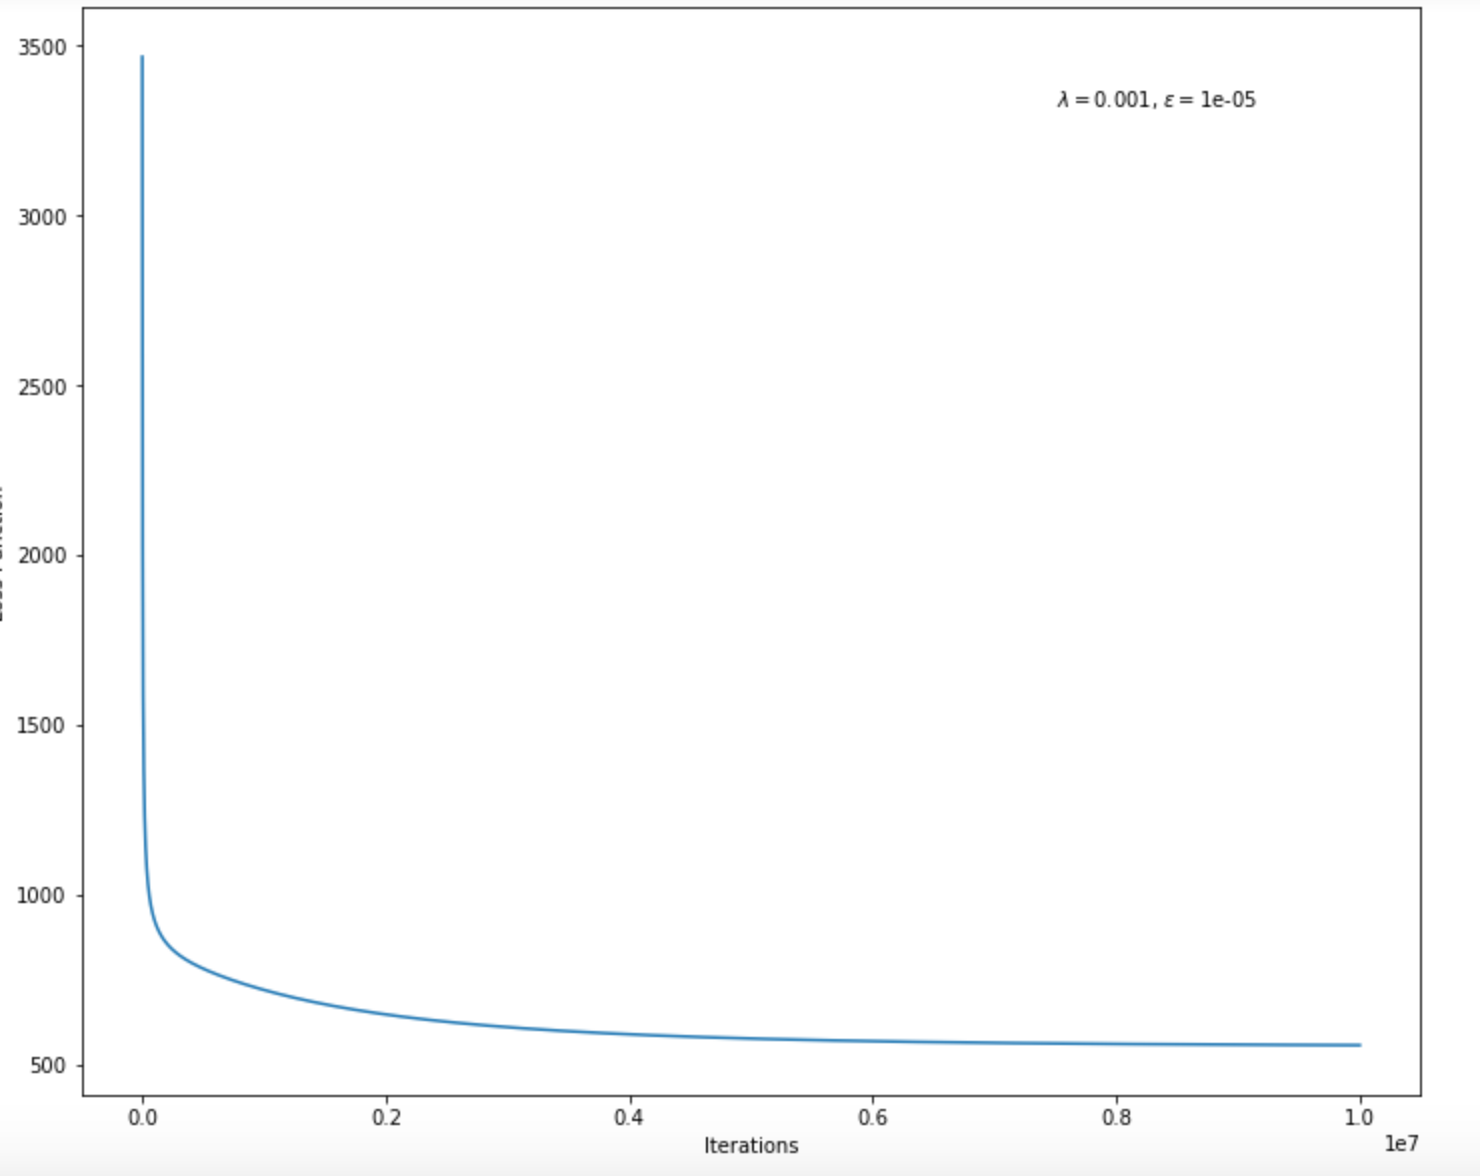
\includegraphics[width=10cm]{LossVsIter_BatchGradDesc}
\end{center}

\subsection*{2.)}

For stochastic gradient descent we use a similar procedure, but now use the update rule 
$$ w \leftarrow w - \epsilon(2 \lambda w - X_i^T(y_i-s_i)). $$
Here, $X_i$ is now a single randomly chosen data point, $y_i$ is the classification of that point.

The relationship of the loss function per iteration is now given in the following plot (using hyperparameters $\lambda, \epsilon$ again chosen through validation). \\
\begin{center}
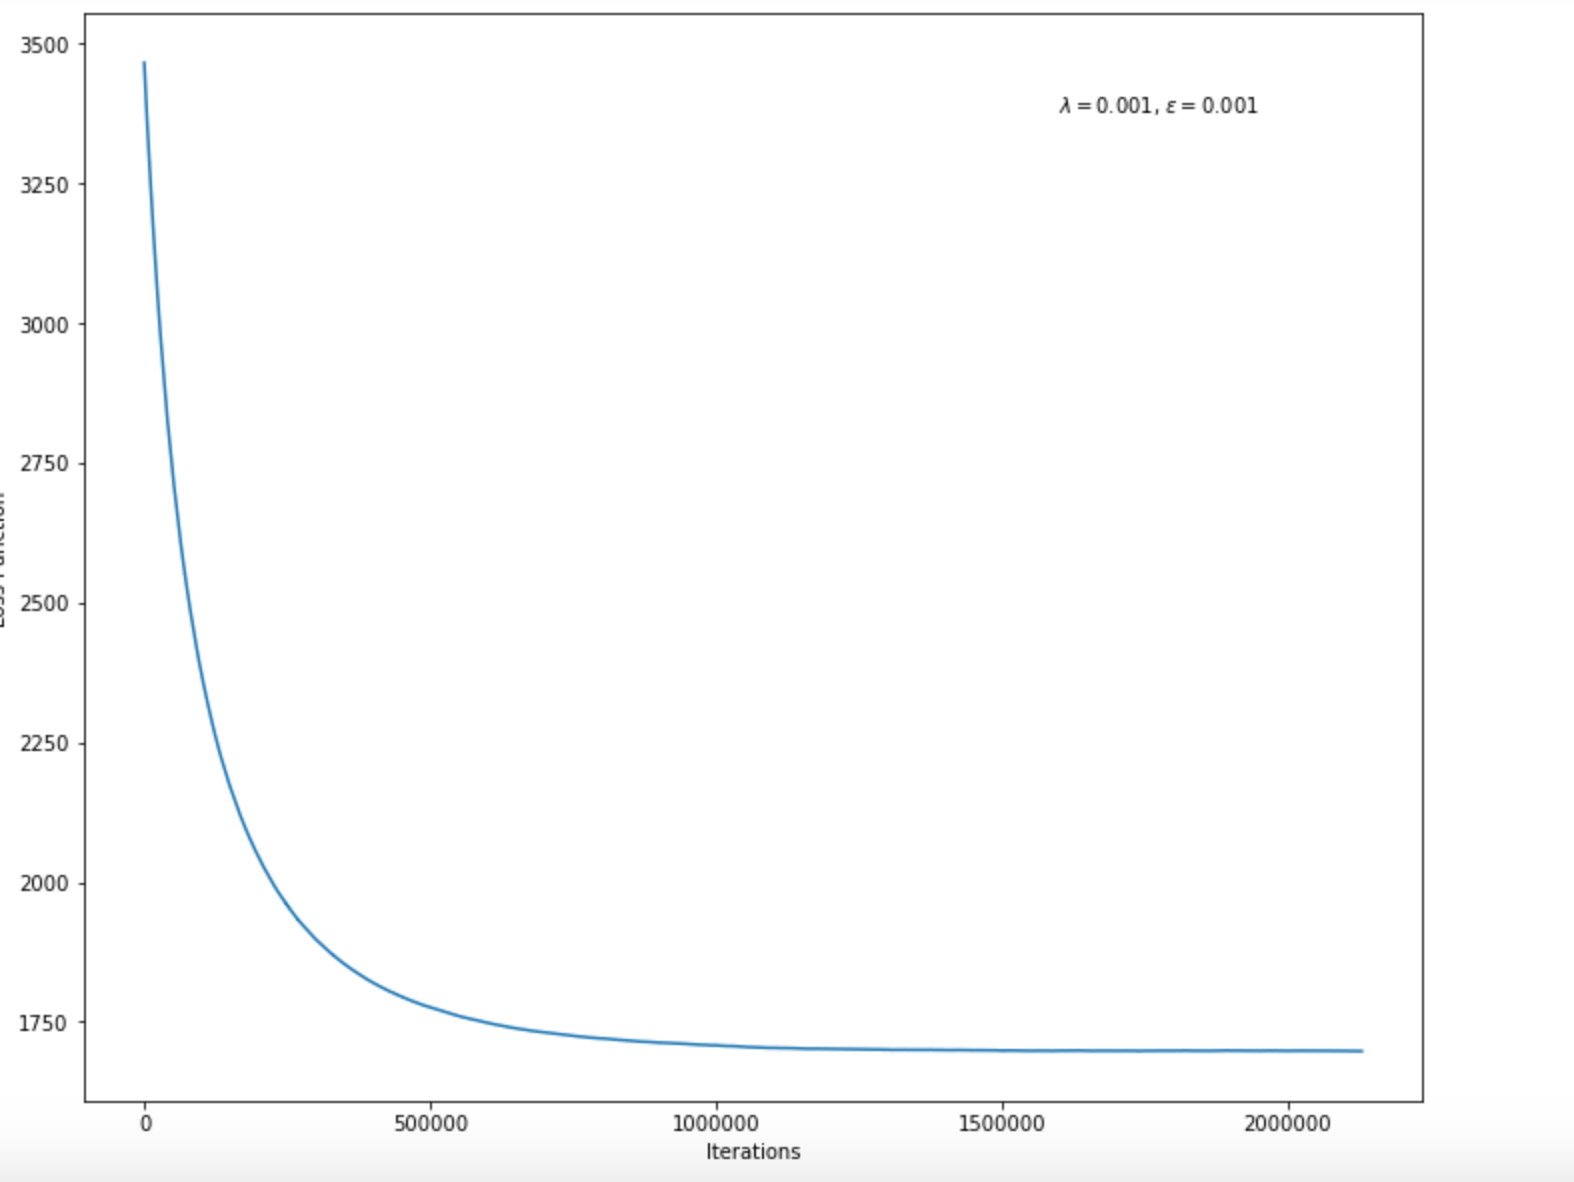
\includegraphics[width=10cm]{LossVsIter_StochGradDesc}
\end{center}

We see here that the convergence of the loss function occurs much faster for stochastic gradient descent.


\subsection*{3.)}

Now, when the learning rate decreases proportionally to $1/t$, we find
\begin{center}
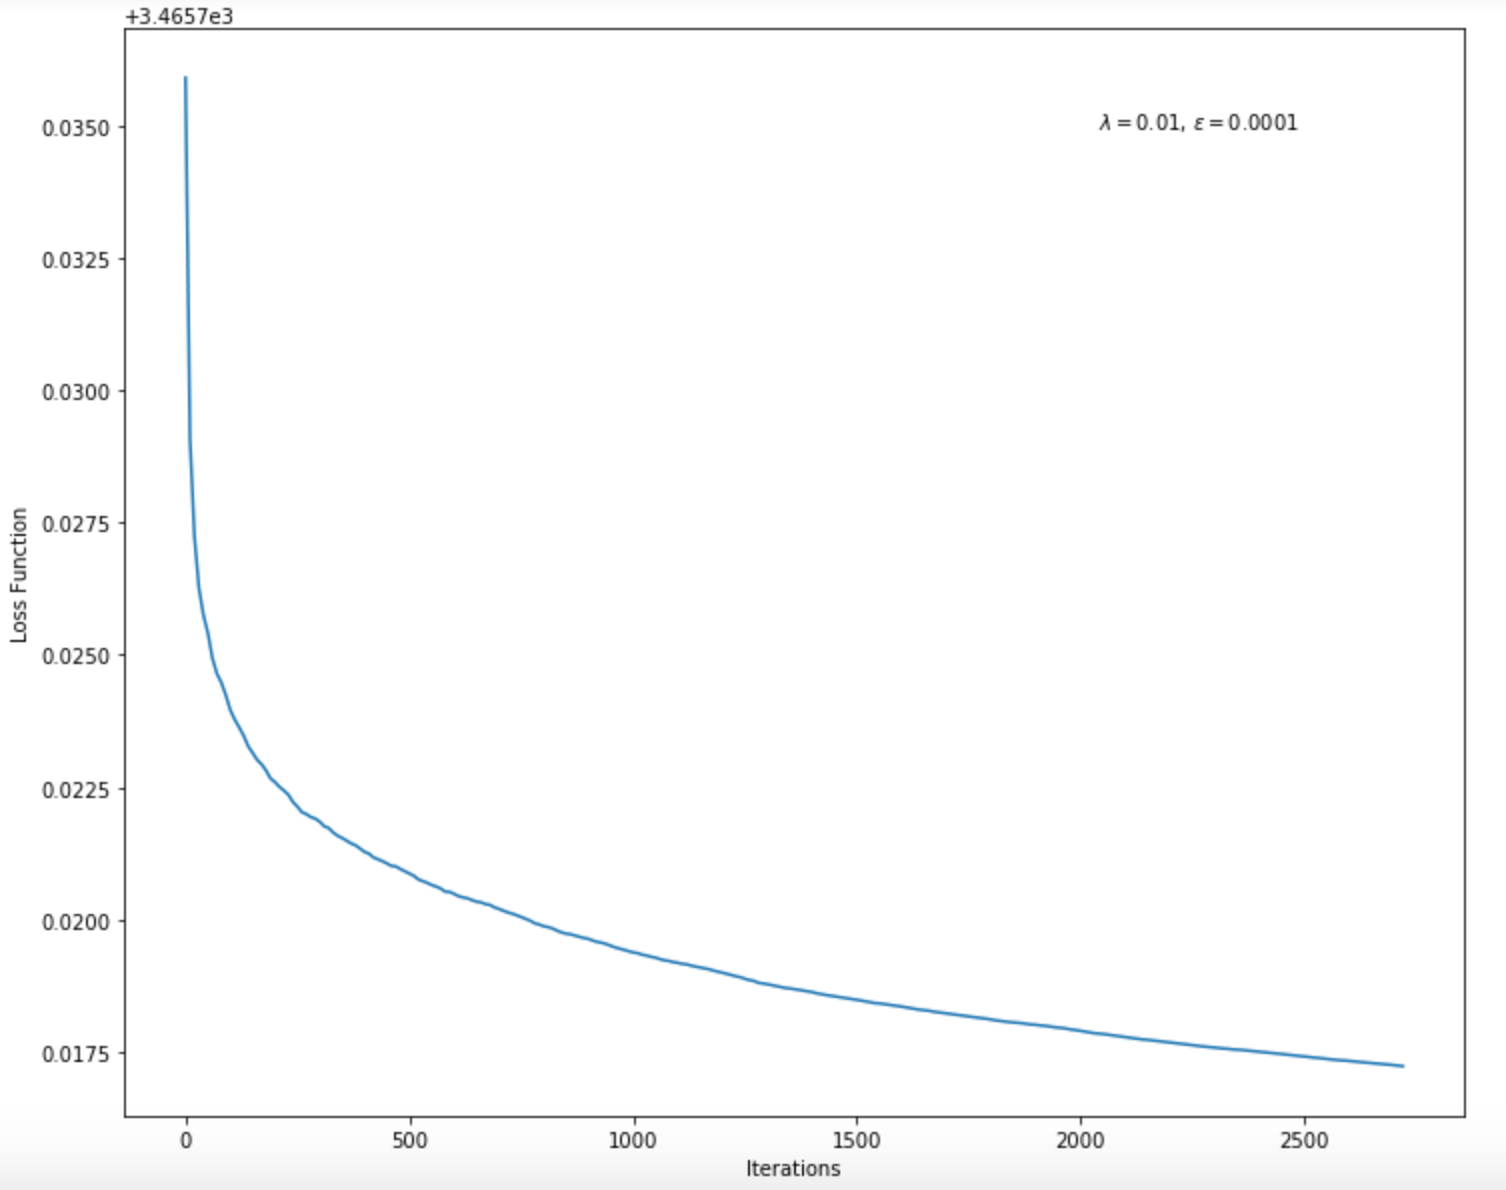
\includegraphics[width=10cm]{LossVsIter_StochGradDesc_deceps}
\end{center}


\subsection*{4.)}

Hyperparameters were chosen using validation (sampling from values of $\lambda$ and $\epsilon$ spaced evenly on a logarithmic scale from $1\times10^{-3} \leq \lambda \leq 10$ and $1\times10^{-5} \leq \epsilon \leq 1\times10^{-3}$). The regularization parameter was chosen to be $\lambda = 0.001$ and $\epsilon = 0.001$.  Notably, on the first Kaggle submission my score was significantly lower than my predicted scores (12\% error as opposed to 3\% training error). After hypothesizing that this difference was likely due to a low regularization parameter causing overfitting to the training data, I chose a larger regularization parameter ($\lambda = ... $\\

Kaggle Submission:\\
\tab Username: \textbf{mnegus}\\
\tab Score:\hspace{0.85cm}\textbf{95.565\%}\\


%%%%%%%%%%%%%%%%%%%%%%%%%%%%%%%%%% PROBLEM 4 %%%%%%%%%%%%%%%%%%%%%%%%%%%%%%%%%%
\newpage
\section*{Problem 5}

If the spike in spam takes place both immediately before and after midnight, then by adding a feature of number of milliseconds since previous midnight, the values of this feature indicating spam will be both small (just a few milleseconds right after midnight) and very large (approximately 86.4 million right before the next midnight). A linear SVM will not be able to construct a margin that separates these two "spam" groups of points from those classified as "ham." 

To remedy this issue, Daniel could change his feature so that it is simply the number of milliseconds from the closest midnight (in either direction, before or after). Then, to improve separation from these points (as a linear classifier will still struggle to separate this grouping from the remainder of data points), Daniel could add a feature being the square of the number of milliseconds from the closest midnight. Then the data would form a paraboloid with number of seconds from midnight being near the minimum, which would allow a linear SVM to easily separate points near midnight. 






\end{document}












